In \cite{Paper1} the authors designed and developed a GPU-based fast Motion Estimation (ME) algorithm and implemented it based on the H.264 JM 14.2 reference software. 
Their goal was to harness the GPU parallel capabilities by breaking off dependencies with tiling frames and than examine how to trade-off the speed-up with Rate Distortion (RD) performance.\\
For that purpose they implemented Motion Estimation on the GPU based on \textit{simplified unsymmetrical multihexagon search \\(smpUMHexagonS)} \cite{yi2005improved}, 
which is one of the fast ME algorithms adopted by the H.264 JM reference software. 
They selected smpUMHexagonS because it can archieve very good tradeoff between computational complexity and coding efficiency. 
It is not only reported to achieve up to 94\% reduction in execution time in ME on a Pentium 4 with comparable RD efficiency, 
when compared with the fast full search in the JM software \cite{yi2005improved}, but also to be very compact and 
therefore meeting the memory constraint of the GPU. Although full search is usually not used in encoding, due its inefficiency, 
the comparison shows, that the compact size of the algorithm is rather important to execute it on the GPU.\\
%
\\
The main problem of ME on the GPUs is the dependency between the different blocks. To find MVs the smpUMHexagonS algorithm is always calculating the minimal Langrangian cost $D + \lambda R$, where D is the sum of
absolute differences (SAD) between the current block and the candidate, and R is the bitrate
to encode the MV dependencies between neighbouring blocks. This implicates a certain dependency between neighbouring blocks. This however is the main reason, why parallelization of ME is very difficult to realise.
The authors of this paper took an easy approach to avoid this problem by just ignoring some dependencies. 
By doing so they set every MV on a tiles boarder to zero and therefore are not always able to calculate the best MVs, resulting in a loss of quality. Another drawback is, 
that the motion vector prediction of the algorithm can't fully be utilized due to the fact, that MVs of neighbouring tiles are unknown. 
It seems that the authors focused their algorithm optimization on the possible speed-up of tiling regardless the quality of the encoded video.\\
\\
The tiling of a frame is presented in figure \ref{tiling}. Each tile consists of \textit{K x L} macroblocks and is to be processed by a single GPU thread concurrent with the other tiles. 
the number of tiles per frame is therefore dependent on the variables \textit{K} and \textit{L}, which describe the width and the hight of each tile.

\begin{figure}[H]
\centerline{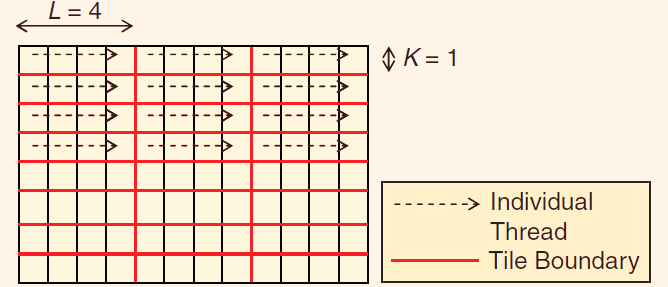
\includegraphics[scale=0.35]{pics/tiling}} % The bounding box is set manually in this example. Useful for some .pdf figures.
\caption{\label{tiling}{\it GPU-based fast ME: the current frame is divided into
multiple tiles to facilitate parallel processing in ME. Here each square represents an MB. (taken from \cite{Paper1})}}
\end{figure}
